\documentclass[10pt, reqno]{amsart}
\usepackage[margin = 0.5 in]{geometry}
\usepackage{multicol}
\usepackage{float}
\usepackage{fancyhdr}
\usepackage{graphicx}
\usepackage{hyperref}
\usepackage{fancyvrb}

\setlength{\abovecaptionskip}{5pt plus 3pt minus 3pt}

\hypersetup{colorlinks=true,allcolors=blue}
\pagestyle{fancy} \fancyhead{} \fancyfoot[C]{\normalsize\thepage}
\renewcommand{\headrulewidth}{0pt}
\begin{document}
\title{ME 5311 \quad Assignment 2 \quad Jacob Ivanov}

\maketitle

\begin{multicols}{2}
Simpson's Rule for numerical integration can be derived from Lagrange's Interpolating Polynomials by constructing the Lagrange Polynomial for 3 points:
\begin{equation}
\begin{aligned}
    f(x) = &+\frac{f_0(x_1-x)(x_2-x)}{(x_1-x_0)(x_2-x_0)}\\
    &+\frac{f_1(x_0-x)(x_2-x)}{(x_0-x_1)(x_2-x_1)}\\
    &+\frac{f_2(x_0-x)(x_1-x)}{(x_0-x_2)(x_1-x_2)}
\end{aligned}
\end{equation}
Integrating $f(x)$ on the domain of $[x_0, x_2]$ is algebraically intense, but otherwise straightforward. Wolfram Mathematica was utilized to make those algebraic simplifications. The console can be seen below:

\begin{figure}[H]
    \centering
    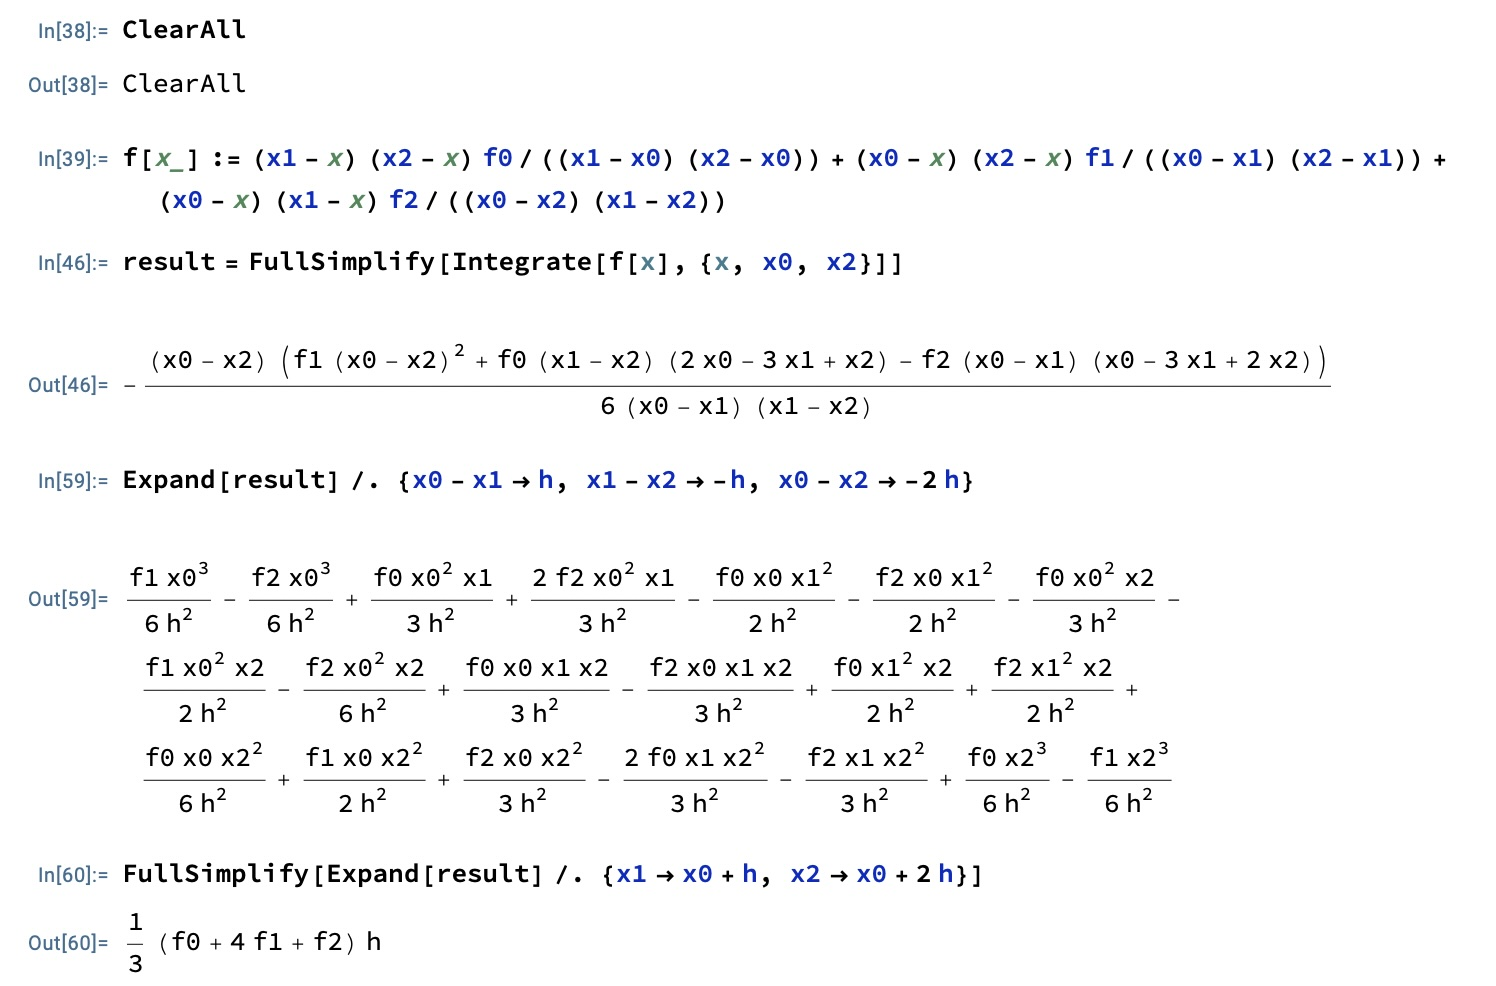
\includegraphics[width=1\linewidth]{Simpson's Rule Derivation.jpg}
    \label{fig:1}
\end{figure}

Simpson's Integration was implemented with C, and the numerical error for the integral $\int_0^\pi \sin(x) \, \mathrm{d}x = 2$ for a $\Delta x = \pi/16$ was $0.00001659104793549915$.

The error was calculated for a $\Delta x = \pi/2^n$ where $n \in \{2, 3, ..., 30\}$ and the convergence was found to be 4th order (up to $N \approx 10^4$, where floating point errors start building up). This can also be seen by plotting this on a loglog plot.

\begin{figure}[H]
    \centering
    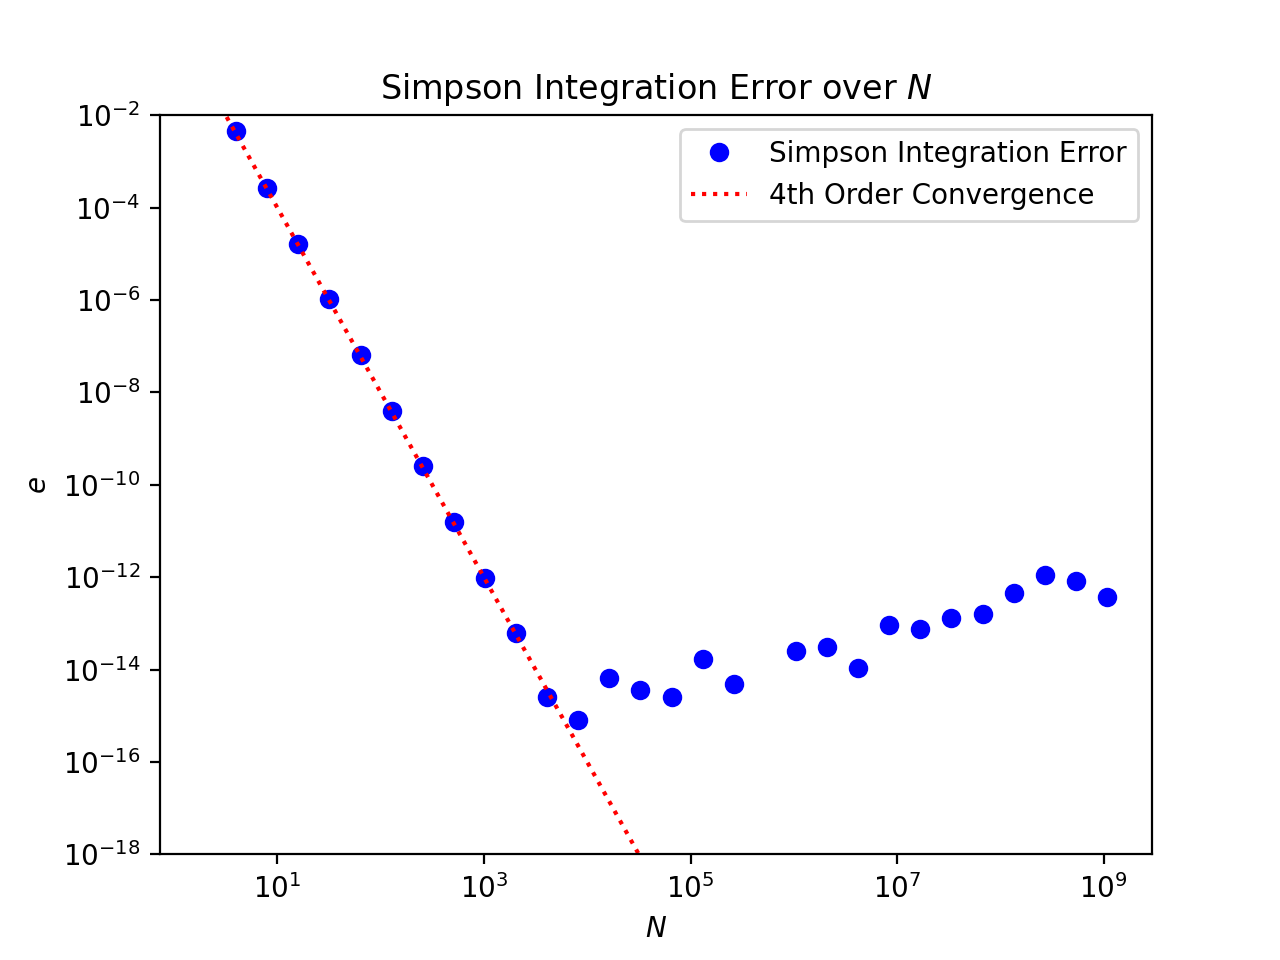
\includegraphics[width=1\linewidth]{Simpson Integration Error over N.png}
    \label{fig:1}
\end{figure}

\end{multicols}

\end{document}